%%%%%%%%%%%%%%%%%%%%%%%%%%%%%%%%%%%%%%%%%
% Beamer Presentation
% LaTeX Template
% Version 1.0 (10/11/12)
%
% This template has been downloaded from:
% http://www.LaTeXTemplates.com
%
% License:
% CC BY-NC-SA 3.0 (http://creativecommons.org/licenses/by-nc-sa/3.0/)
%
%%%%%%%%%%%%%%%%%%%%%%%%%%%%%%%%%%%%%%%%%

%----------------------------------------------------------------------------------------
%	PACKAGES AND THEMES
%----------------------------------------------------------------------------------------

\documentclass{beamer}

\mode<presentation> {

% The Beamer class comes with a number of default slide themes
% which change the colors and layouts of slides. Below this is a list
% of all the themes, uncomment each in turn to see what they look like.

%\usetheme{default}
%\usetheme{AnnArbor}
%\usetheme{Antibes}
%\usetheme{Bergen}
%\usetheme{Berkeley}
%\usetheme{Berlin}
%\usetheme{Boadilla}
%\usetheme{CambridgeUS}
%\usetheme{Copenhagen}
%\usetheme{Darmstadt}
%\usetheme{Dresden}
%\usetheme{Frankfurt}
%\usetheme{Goettingen}
%\usetheme{Hannover}
%\usetheme{Ilmenau}
%\usetheme{JuanLesPins}
%\usetheme{Luebeck}
    \usetheme{Madrid}
%\usetheme{Malmoe}
%\usetheme{Marburg}
%\usetheme{Montpellier}
%\usetheme{PaloAlto}
%\usetheme{Pittsburgh}
%\usetheme{Rochester}
%\usetheme{Singapore}
%\usetheme{Szeged}
%\usetheme{Warsaw}

% As well as themes, the Beamer class has a number of color themes
% for any slide theme. Uncomment each of these in turn to see how it
% changes the colors of your current slide theme.

%\usecolortheme{albatross}
%\usecolortheme{beaver}
%\usecolortheme{beetle}
%\usecolortheme{crane}
%\usecolortheme{dolphin}
%\usecolortheme{dove}
%\usecolortheme{fly}
%\usecolortheme{lily}
%\usecolortheme{orchid}
%\usecolortheme{rose}
%\usecolortheme{seagull}
%\usecolortheme{seahorse}
%\usecolortheme{whale}
%\usecolortheme{wolverine}

%\setbeamertemplate{footline} % To remove the footer line in all slides uncomment this line
%\setbeamertemplate{footline}[page number] % To replace the footer line in all slides with a simple slide count uncomment this line

%\setbeamertemplate{navigation symbols}{} % To remove the navigation symbols from the bottom of all slides uncomment this line
}

\usepackage{graphicx} % Allows including images
\usepackage{booktabs} % Allows the use of \toprule, \midrule and \bottomrule in tables
\usepackage{mystyle}
\usepackage{lmodern}

%----------------------------------------------------------------------------------------
%	TITLE PAGE
%----------------------------------------------------------------------------------------

\title[Stokes Flow]{Mixed Element Methods for Stokes Equations} % The short title appears at the bottom of every slide, the full title is only on the title page

\author{Will Frey} % Your name
\institute[VA Tech] % Your institution as it will appear on the bottom of every slide, may be shorthand to save space
{
    Virginia Tech \\ % Your institution for the title page
}
\date{\today} % Date, can be changed to a custom date

\begin{document}

\begin{frame}
    \titlepage% Print the title page as the first slide
\end{frame}

\begin{frame}
    \frametitle{Overview} % Table of contents slide, comment this block out to remove it
    \tableofcontents % Throughout your presentation, if you choose to use \section{} and \subsection{} commands, these will automatically be printed on this slide as an overview of your presentation
\end{frame}

%-----------------------------------------------------------------------------
%	PRESENTATION SLIDES
%-----------------------------------------------------------------------------

%------------------------------------------------
\section{Theory} % Sections can be created in order to organize your presentation into discrete blocks, all sections and subsections are automatically printed in the table of contents as an overview of the talk
%------------------------------------------------

\begin{frame}
    \frametitle{Stokes Equations}
    \begin{block}{Stokes with Homogeneous Boundary and Zero-Mean Pressure}
        \begin{equation}
            \begin{split}
                -\text{Re}^{-1}\,\del^2 u_1 + \frac{\p}{\p x} u_1 &= f_1 \quad
                    \text{in } \Omega, \\
                -\text{Re}^{-1}\,\del^2 u_2 + \frac{\p}{\p y} u_2 &= f_2 \quad
                    \text{in } \Omega, \\
                \frac{\p}{\p x} u_1 + \frac{\p}{\p y} u_2 &= 0 \quad \text{in }
                    \Omega, \\
                u_1 &= 0 \quad \text{on } \p \Omega, \\
                u_2 &= 0 \quad \text{on } \p \Omega, \\
                \int p(x,y) \,d\Omega &= 0 \quad \text{on } \Omega.
            \end{split}
        \end{equation}
    \end{block}

    I take $\text{Re} = 1$.
\end{frame}

%------------------------------------------------

\begin{frame}
    \frametitle{Mixed Elements}
    \begin{columns}[c] % The "c" option specifies centered vertical alignment while the "t" option is used for top vertical alignment

        \column{.45\textwidth} % Left column and width
        \textbf{Framework}
        \begin{enumerate}
            \item $\vect{u} \in H_{0}^{1}{(\Omega)}^2$
            \item $H_{0}^{1}{(\Omega)}^2 = \left\{(u_1, u_2) : u_i \in
                    H_{0}^{1}(\Omega)\right\}$
            \item $p \in L_{0}^{2}(\Omega)$
            \item $L_{0}^{2}(\Omega) = \left\{p \in L^2 : \int p\,d\Omega =
                0\right\}$
            \item Look for solution in $H_{0}^{1}{(\Omega)}^2 \times
                L_{0}^{2}(\Omega)$
        \end{enumerate}

        \column{.5\textwidth} % Right column and width
        We break up the function spaces for velocity $\vect{u}$ and pressure
        $p$ into two distinct Hilbert spaces. We then choose appropriate finite
        dimensional subspaces to find our finite element solution. I chose the
        \textbf{Taylor-Hood} $\mathbb{P}_2 - \mathbb{P}_1$ finite element.

    \end{columns}
\end{frame}
\begin{frame}
    \frametitle{Taylor-Hood Finite Element}
    \begin{figure}
        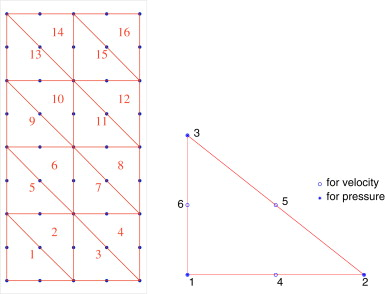
\includegraphics[width=0.3\linewidth]{./taylorhood.jpg}
        \caption{The $\mathbb{P}_2 - \mathbb{P}_1$ Element}
    \end{figure}
\end{frame}


%------------------------------------------------

\begin{frame}
    \frametitle{Variatonal Weak Form}
    \begin{block}{Variational Formulation}
        Find $\vect{u} \in H_{0}^{1}{(\Omega)}^2$ and $p \in L_{0}^{2}(\Omega)$
        so that
        \begin{equation}
            \begin{split}
                \left( \del \vect{u}, \del \vect{v} \right) + \left( p, \del
                    \cdot \vect{v} \right) &= \left(\vect{f}, \vect{v} \right)
                    \quad \text{for all } \vect{v} \in H_{0}^{1}
                    {(\Omega)}^{2}, \\
                -\left(\del \cdot \vect{u}, q \right) &= 0  \qquad \text{for
                    all } q \in{L}_{0}^{2} (\Omega).
            \end{split}
        \end{equation}
    \end{block}
\end{frame}


\begin{frame}
    \frametitle{Variational Weak Form Cont'd}
    Find $(u_{1,h}, u_{2,h}) \in V_h \subset H_{0}^{1}(\Omega)^2$ and $p_h \in
    Q_h \subset L_{0}^{2} (\Omega)$ such that
\begin{equation}
    \begin{split}
        \int \del u_{1,h} \cdot \del v_{1,h} \,d\Omega - \int p_h \frac{\p
            v_{1,h}}{\p x} \,d\Omega &= \int f_1 v_{1,h} \,d\Omega \qquad
            \forall v_{1,h} \in V_h, \\
        \int \del u_{2,h} \cdot \del v_{2,h} \,d\Omega - \int p_h \frac{\p
            v_{2,h}}{\p y} \,d\Omega &= \int f_2 v_{2,h} \,d\Omega \qquad
            \forall v_{2,h} \in V_h \text{ and }, \\
        \int \left(\frac{\p u_{1,h}}{\p x} + \frac{\p u_{2,h}}{\p y}\right) q_h
            \,d\Omega &= 0 \qquad \forall q_h \in Q_h.
    \end{split}
\end{equation}
\end{frame}


\begin{frame}
    \frametitle{Conditions for Well-Posedness}
    We get a system of the form
    $\begin{bmatrix}
        A & B \\
        B^T & 0
    \end{bmatrix}
    \begin{bmatrix}
        u \\
        v
    \end{bmatrix}
    =
    \begin{bmatrix}
        f \\
        0
    \end{bmatrix}.$

    \begin{block}{Ladyzenskaya-Babuska-Breezi Condition (LBB)}
        A solution exists if and only if
        \[\inf_{v \in V} \sup_{u \in U} \frac{a(u, v)}{\norm{u}\norm{v}} >
            \alpha_E > 0 \]
        and the solution is unique if and only if \[\inf_{u
            \in U} \sup_{v \in V} \frac{(a(u, v)}{\norm{u}\norm{v}} > \alpha_U
            > 0 \]
        for a generic bilinear form $a(\cdot,\cdot): U \times V \to \R$ defined
        on the Cartesian product of Hilbert spaces $U \times V$.
    \end{block}

\end{frame}

\begin{frame}
    \frametitle{Error Estimate}
    \begin{block}{Stokes Error Estimate}
        Let $V_h \times Q_h$ satisfy the LBB conditions with polynomials of
        order max order $k$ in $V_h$ and $l$ in $Q_h$. Let $u \in
        H^{k+1}(\Omega)^2$ and $p \in L^2(\Omega)$ be the solution of the
        Stokes equation. Then
        \begin{equation}
            \norm{\del (v - v_h)} + \norm{p - p_h} \leq C h^{\min \{k, l+1\}}
            (\norm{\del^{k+1}v} + \norm{\del^l p}).
        \end{equation}
    \end{block}

    We see that the error is optimal for both spaces when $k = l + 1$. This is
    why $\mathbb{P}_2 - \mathbb{P}_1$ works.
\end{frame}


\section{Numerical Results}

\begin{frame}
    \frametitle{$f_1(x,y) = y, f_2(x,y) = -x$}
\begin{figure}
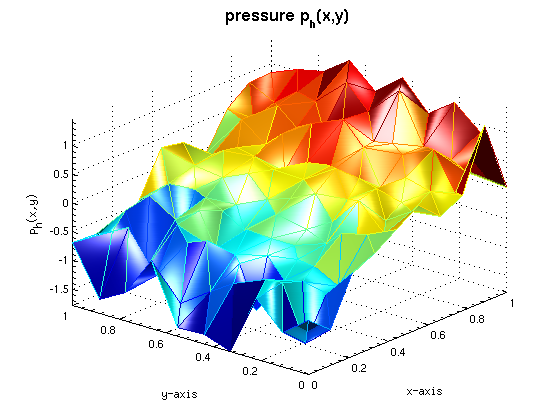
\includegraphics[width=0.5\linewidth]{./p1.png}
\caption{$p_h$ for $h=0.1$}
\end{figure}
\end{frame}

\begin{frame}
    \frametitle{$f_1(x,y) = y, f_2(x,y) = -x$}
\begin{figure}
    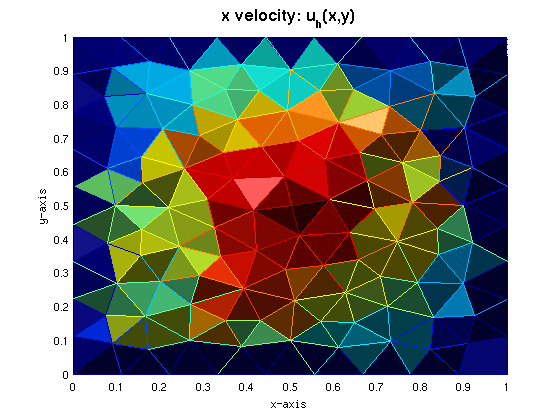
\includegraphics[width=0.5\linewidth]{./magu_1.png}
\caption{$\abs{u_h}$ for $h=0.1$}
\end{figure}
\end{frame}

\begin{frame}
    \frametitle{$f_1(x,y) = y, f_2(x,y) = -x$}
\begin{figure}
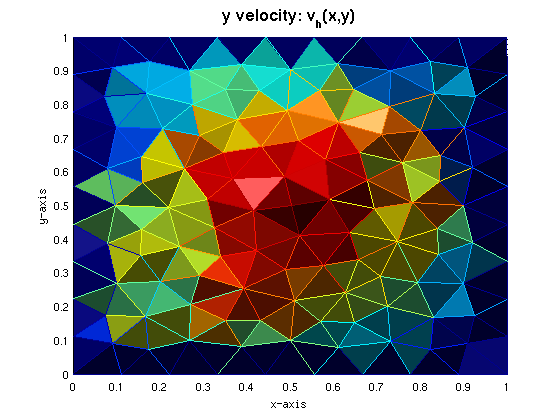
\includegraphics[width=0.5\linewidth]{./magv_1.png}
\caption{$\abs{v_h}$ for $h=0.1$}
\end{figure}
\end{frame}


\begin{frame}
    \frametitle{$f_1(x,y) = y, f_2(x,y) = -x$}
\begin{figure}
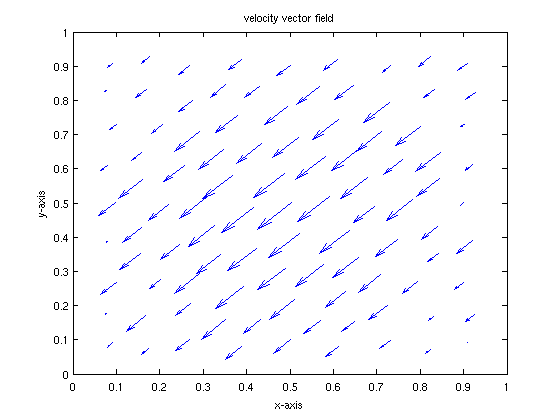
\includegraphics[width=0.5\linewidth]{./q1.png}
\caption{Quiver Plot for $h=0.1$}
\end{figure}
\end{frame}


\begin{frame}
    \frametitle{$f_1(x,y) = y, f_2(x,y) = -x$}
\begin{figure}
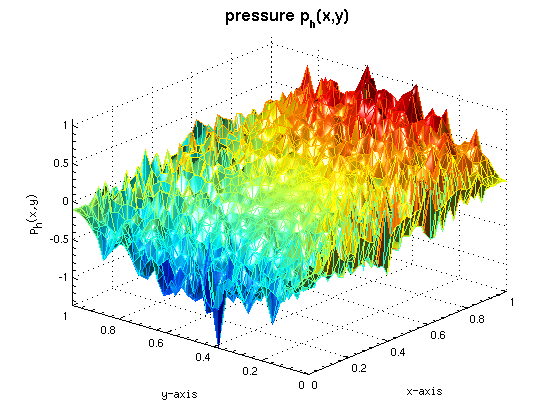
\includegraphics[width=0.5\linewidth]{./p2.png}
\caption{$p_h$ for $h=0.025$}
\end{figure}
\end{frame}

\begin{frame}
    \frametitle{$f_1(x,y) = y, f_2(x,y) = -x$}
\begin{figure}
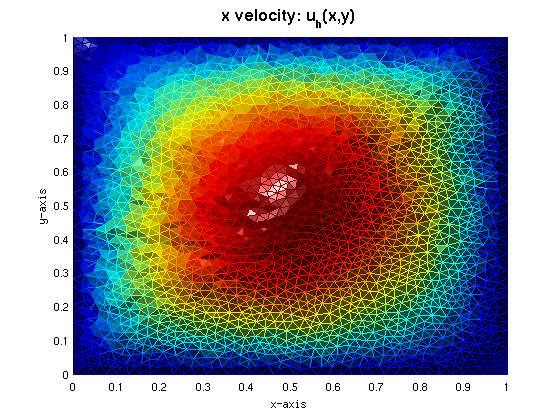
\includegraphics[width=0.5\linewidth]{./magu_2.png}
\caption{$\abs{u_h}$ for $h=0.025$}
\end{figure}
\end{frame}

\begin{frame}
    \frametitle{$f_1(x,y) = y, f_2(x,y) = -x$}
\begin{figure}
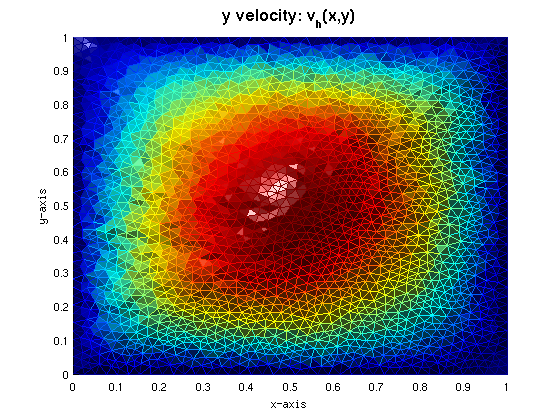
\includegraphics[width=0.5\linewidth]{./magv_2.png}
\caption{$\abs{v_h}$ for $h=0.025$}
\end{figure}
\end{frame}

\begin{frame}
    \frametitle{$f_1(x,y) = y, f_2(x,y) = -x$}
\begin{figure}
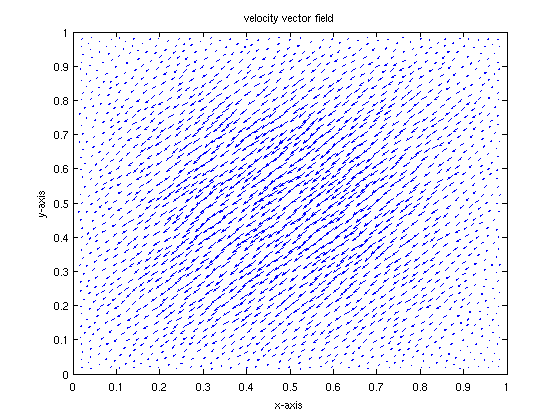
\includegraphics[width=0.5\linewidth]{./q2.png}
\caption{Quiver Plot for $h=0.025$}
\end{figure}
\end{frame}


\begin{frame}
    \frametitle{$f_1(x,y) = x^2 y^3 \cos(\pi y), f_2(x,y) = 1\text{e}-4 \cdot
    \abs{y - 0.5}$}
\begin{figure}
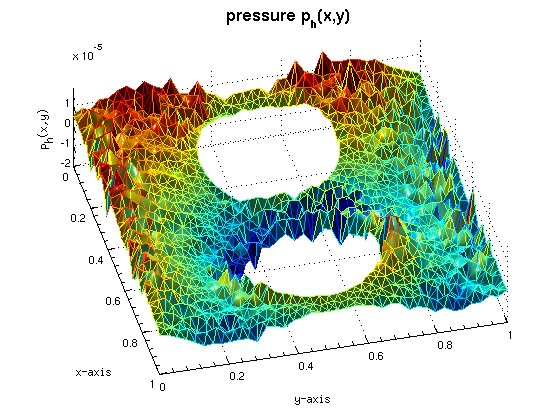
\includegraphics[width=0.5\linewidth]{./p3.png}
\caption{$p_h$ for $h=0.025$}
\end{figure}
\end{frame}

\begin{frame}
    \frametitle{$f_1(x,y) = x^2 y^3 \cos(\pi y), f_2(x,y) = 1\text{e}-4 \cdot
    \abs{y - 0.5}$}
\begin{figure}
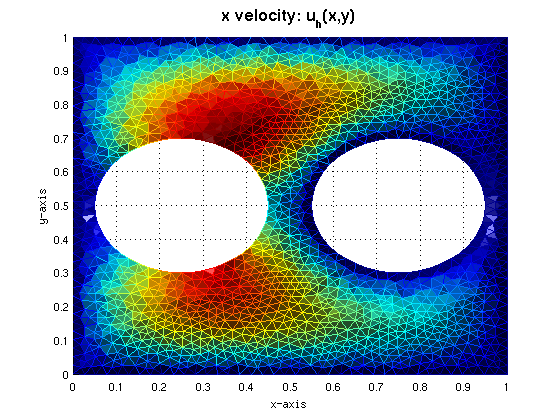
\includegraphics[width=0.5\linewidth]{./magu_3.png}
\caption{$\abs{u_h}$ for $h=0.025$}
\end{figure}
\end{frame}

\begin{frame}
    \frametitle{$f_1(x,y) = x^2 y^3 \cos(\pi y), f_2(x,y) = 1\text{e}-4 \cdot
    \abs{y - 0.5}$}
\begin{figure}
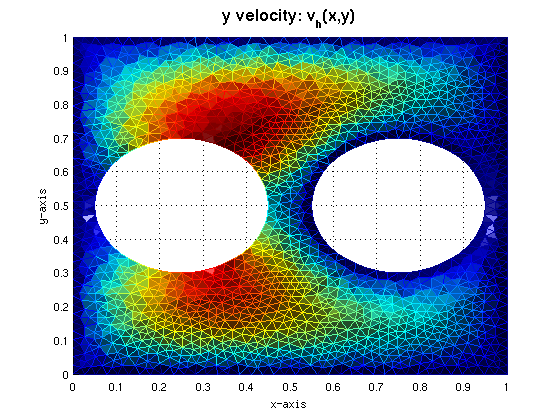
\includegraphics[width=0.5\linewidth]{./magv_3.png}
\caption{$\abs{v_h}$ for $h=0.025$}
\end{figure}
\end{frame}

\begin{frame}
    \frametitle{$f_1(x,y) = y, f_2(x,y) = -x$}
\begin{figure}
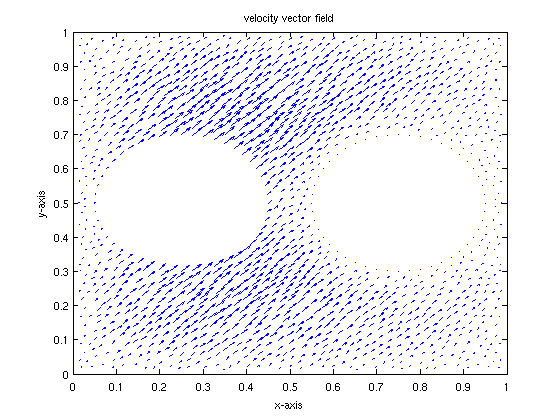
\includegraphics[width=0.5\linewidth]{./q3.png}
\caption{Quiver Plot for $h=0.025$}
\end{figure}
\end{frame}
%------------------------------------------------

\begin{frame}[shrink=30]
    \frametitle{References}
    \footnotesize{
        \begin{thebibliography}{99}

                \bibitem[Braess, 2006]{br}
                Dietrich Braess,
                \newblock%
                \emph{Finite elements: Theory, fast solvers, and
                applications in solid mechanics},
                \newblock%
                Cambridge University Press,
                Third Edition,
                2006.

                \bibitem[{Girault \& Raviart, 1986}]{vp}
                Vivette Girault and Pierre-Arnaud Raviart,
                \newblock%
                \emph{Finite Element Methods for Navier-Stokes Equations:
                Theory and Algorithms},
                \newblock%
                Springer-Verlag, Germany, 1986.

                \bibitem[Johnson, 2009]{j}
                Claes Johnson,
                \newblock%
                \emph{Numerical Solution to Partial Differential Equations
                by the Finite Element Method},
                \newblock%
                Dover, Mineola, New York, 2009.

                \bibitem[Kim et al., 2006]{nm}
                Sang Dong Kim, Yong Hun Lee, and Byeong Chun Shin,
                \newblock%
                \emph{Newton's Method for the Navier-Stokes Equations with
                Finite-Element Initial Guess of Stokes Equation},
                \newblock%
                Computers and Mathematics with Applications 51 (2006), pp.
                805--816.

                \bibitem[{Dennis \& Schnabel, 1983}]{ds}
                J.E. Dennis, Jr.\'and Robert B. Schnabel,
                \newblock%
                \emph{Numerical Methods for Unconstrained Optimization and
                Nonlinear Equations},
                \newblock%
                Prentice-Hall, Inc, Englewood Cliffs, New Jersey, 1983.

                \bibitem[Ciarlet]{c}
                Philippe G. Ciarlet,
                \newblock%
                \emph{The Finite Element Method for Elliptic Problems},
                \newblock%
                North Holland Publishing Company, Volume 4, 1978.
        \end{thebibliography}
    }
\end{frame}

%------------------------------------------------

\begin{frame}
    \Huge{\centerline{The End}}
\end{frame}

%----------------------------------------------------------------------------------------

\end{document} 
